\documentclass[tikz, border=2pt]{standalone}
\usepackage{amsmath}

\begin{document}
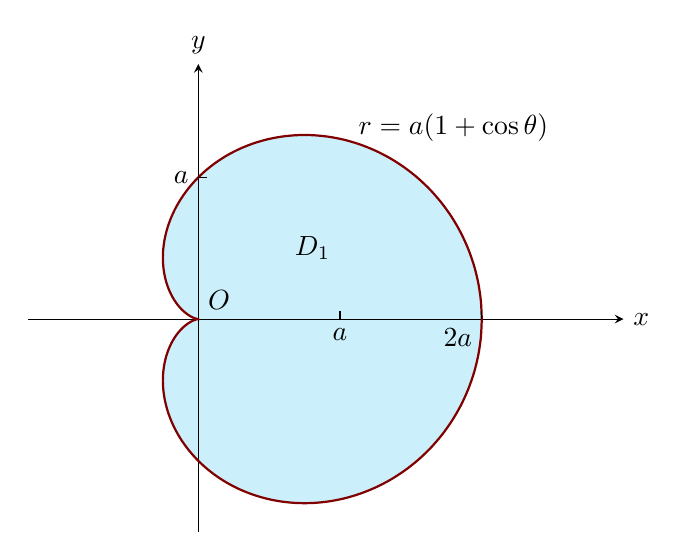
\begin{tikzpicture}[scale=1.8, >=stealth]
    % 定义常数 a = 1
    \def\a{1}
    
    % 填充心形线内部区域
    \fill[cyan!20] plot[domain=0:2*pi, smooth, samples=100]
        ({\a*(1+cos(\x r))*cos(\x r)}, {\a*(1+cos(\x r))*sin(\x r)}) -- cycle;
    
    % 画坐标轴
    \draw[->] (-1.2,0) -- (3.0,0) node[right] {$x$};
    \draw[->] (0,-1.5) -- (0,1.8) node[above] {$y$};
    
    % 画心形线轮廓
    \draw[thick, red!50!black] plot[domain=0:2*pi, smooth, samples=100]
        ({\a*(1+cos(\x r))*cos(\x r)}, {\a*(1+cos(\x r))*sin(\x r)});
    
    % 在 x 轴上标注 a 和 2a
    \draw[dashed] (\a,0) -- (\a,0.1) ;
    \draw[dashed] (2*\a,0) -- (2*\a,0.1) ;
    % 在 y 轴上标注 a
    \draw[dashed] (0,\a) -- (0.1,\a);
  
    
    % 标注极点
    \node[above right] at (0,0) {$O$};
   \node[below] at (\a,0) {$a$};
   \node[below left] at (2*\a, 0) {$2a$};
   \node[left] at (0,\a) {$a$};
   \node[left] at (\a, \a / 2) {$D_1$};
    
    % 标注曲线方程
    \node at (1.8,1.35) {$r = a(1+\cos\theta)$};
\end{tikzpicture}
\end{document}